\documentclass[]{report}
\usepackage{lmodern}
\usepackage{amssymb,amsmath}
\usepackage{ifxetex,ifluatex}
\usepackage{fixltx2e} % provides \textsubscript
\ifnum 0\ifxetex 1\fi\ifluatex 1\fi=0 % if pdftex
  \usepackage[T1]{fontenc}
  \usepackage[utf8]{inputenc}
\else % if luatex or xelatex
  \ifxetex
    \usepackage{mathspec}
  \else
    \usepackage{fontspec}
  \fi
  \defaultfontfeatures{Ligatures=TeX,Scale=MatchLowercase}
\fi
% use upquote if available, for straight quotes in verbatim environments
\IfFileExists{upquote.sty}{\usepackage{upquote}}{}
% use microtype if available
\IfFileExists{microtype.sty}{%
\usepackage{microtype}
\UseMicrotypeSet[protrusion]{basicmath} % disable protrusion for tt fonts
}{}
\usepackage{hyperref}
\hypersetup{unicode=true,
            pdftitle={PROJECT 2: PREDICTING PH},
            pdfauthor={Juliann McEachern},
            pdfborder={0 0 0},
            breaklinks=true}
\urlstyle{same}  % don't use monospace font for urls
\usepackage{color}
\usepackage{fancyvrb}
\newcommand{\VerbBar}{|}
\newcommand{\VERB}{\Verb[commandchars=\\\{\}]}
\DefineVerbatimEnvironment{Highlighting}{Verbatim}{commandchars=\\\{\}}
% Add ',fontsize=\small' for more characters per line
\usepackage{framed}
\definecolor{shadecolor}{RGB}{248,248,248}
\newenvironment{Shaded}{\begin{snugshade}}{\end{snugshade}}
\newcommand{\AlertTok}[1]{\textcolor[rgb]{0.94,0.16,0.16}{#1}}
\newcommand{\AnnotationTok}[1]{\textcolor[rgb]{0.56,0.35,0.01}{\textbf{\textit{#1}}}}
\newcommand{\AttributeTok}[1]{\textcolor[rgb]{0.77,0.63,0.00}{#1}}
\newcommand{\BaseNTok}[1]{\textcolor[rgb]{0.00,0.00,0.81}{#1}}
\newcommand{\BuiltInTok}[1]{#1}
\newcommand{\CharTok}[1]{\textcolor[rgb]{0.31,0.60,0.02}{#1}}
\newcommand{\CommentTok}[1]{\textcolor[rgb]{0.56,0.35,0.01}{\textit{#1}}}
\newcommand{\CommentVarTok}[1]{\textcolor[rgb]{0.56,0.35,0.01}{\textbf{\textit{#1}}}}
\newcommand{\ConstantTok}[1]{\textcolor[rgb]{0.00,0.00,0.00}{#1}}
\newcommand{\ControlFlowTok}[1]{\textcolor[rgb]{0.13,0.29,0.53}{\textbf{#1}}}
\newcommand{\DataTypeTok}[1]{\textcolor[rgb]{0.13,0.29,0.53}{#1}}
\newcommand{\DecValTok}[1]{\textcolor[rgb]{0.00,0.00,0.81}{#1}}
\newcommand{\DocumentationTok}[1]{\textcolor[rgb]{0.56,0.35,0.01}{\textbf{\textit{#1}}}}
\newcommand{\ErrorTok}[1]{\textcolor[rgb]{0.64,0.00,0.00}{\textbf{#1}}}
\newcommand{\ExtensionTok}[1]{#1}
\newcommand{\FloatTok}[1]{\textcolor[rgb]{0.00,0.00,0.81}{#1}}
\newcommand{\FunctionTok}[1]{\textcolor[rgb]{0.00,0.00,0.00}{#1}}
\newcommand{\ImportTok}[1]{#1}
\newcommand{\InformationTok}[1]{\textcolor[rgb]{0.56,0.35,0.01}{\textbf{\textit{#1}}}}
\newcommand{\KeywordTok}[1]{\textcolor[rgb]{0.13,0.29,0.53}{\textbf{#1}}}
\newcommand{\NormalTok}[1]{#1}
\newcommand{\OperatorTok}[1]{\textcolor[rgb]{0.81,0.36,0.00}{\textbf{#1}}}
\newcommand{\OtherTok}[1]{\textcolor[rgb]{0.56,0.35,0.01}{#1}}
\newcommand{\PreprocessorTok}[1]{\textcolor[rgb]{0.56,0.35,0.01}{\textit{#1}}}
\newcommand{\RegionMarkerTok}[1]{#1}
\newcommand{\SpecialCharTok}[1]{\textcolor[rgb]{0.00,0.00,0.00}{#1}}
\newcommand{\SpecialStringTok}[1]{\textcolor[rgb]{0.31,0.60,0.02}{#1}}
\newcommand{\StringTok}[1]{\textcolor[rgb]{0.31,0.60,0.02}{#1}}
\newcommand{\VariableTok}[1]{\textcolor[rgb]{0.00,0.00,0.00}{#1}}
\newcommand{\VerbatimStringTok}[1]{\textcolor[rgb]{0.31,0.60,0.02}{#1}}
\newcommand{\WarningTok}[1]{\textcolor[rgb]{0.56,0.35,0.01}{\textbf{\textit{#1}}}}
\usepackage{graphicx,grffile}
\makeatletter
\def\maxwidth{\ifdim\Gin@nat@width>\linewidth\linewidth\else\Gin@nat@width\fi}
\def\maxheight{\ifdim\Gin@nat@height>\textheight\textheight\else\Gin@nat@height\fi}
\makeatother
% Scale images if necessary, so that they will not overflow the page
% margins by default, and it is still possible to overwrite the defaults
% using explicit options in \includegraphics[width, height, ...]{}
\setkeys{Gin}{width=\maxwidth,height=\maxheight,keepaspectratio}
\IfFileExists{parskip.sty}{%
\usepackage{parskip}
}{% else
\setlength{\parindent}{0pt}
\setlength{\parskip}{6pt plus 2pt minus 1pt}
}
\setlength{\emergencystretch}{3em}  % prevent overfull lines
\providecommand{\tightlist}{%
  \setlength{\itemsep}{0pt}\setlength{\parskip}{0pt}}
\setcounter{secnumdepth}{0}

%%% Use protect on footnotes to avoid problems with footnotes in titles
\let\rmarkdownfootnote\footnote%
\def\footnote{\protect\rmarkdownfootnote}

%%% Change title format to be more compact
\usepackage{titling}

% Create subtitle command for use in maketitle
\providecommand{\subtitle}[1]{
  \posttitle{
    \begin{center}\large#1\end{center}
    }
}

\setlength{\droptitle}{-2em}

  \title{PROJECT 2: PREDICTING PH}
    \pretitle{\vspace{\droptitle}\centering\huge}
  \posttitle{\par}
    \author{Juliann McEachern}
    \preauthor{\centering\large\emph}
  \postauthor{\par}
      \predate{\centering\large\emph}
  \postdate{\par}
    \date{10 December 2019}

% set plain style for page numbers
\usepackage[margin=1in]{geometry}
\usepackage{fancyhdr}
\pagestyle{fancy}
\fancyhead[LE,RO]{\textbf{Group 2}}
\fancyhead[RE,LO]{\textbf{Project 2: Predicting PH}}
\raggedbottom
\setlength{\parskip}{1em}

% change font
\usepackage{fontspec}
\setmainfont{Arial}

% format titles 
\usepackage{xcolor}
\usepackage{sectsty}
\usepackage{etoolbox}
\usepackage{titling}
\definecolor{prettyblue}{RGB}{84, 144, 240}
\definecolor{bluegray}{RGB}{98, 107, 115}
\pretitle{\begin{center}\Huge\color{prettyblue}\textbf}
\posttitle{\par\LARGE\color{gray}DATA 624 - Predictive Analytics\linebreak Group 2\end{center}}
\preauthor{\begin{center}\large\textbf{Group Members:}\linebreak\textit}
\postauthor{\end{center}}

% Format chapter output
\usepackage{titlesec}
\titleclass{\part}{top}
\titleclass{\chapter}{straight}
\titleformat{\chapter}
  {\normalfont\color{prettyblue}\LARGE\bfseries}{\thechapter}{1em}{}
\titlespacing*{\chapter}{0pt}{3.5ex plus 1ex minus .2ex}{2.3ex plus .2ex}


% create color block quotes
\usepackage{tcolorbox}
\newtcolorbox{myquote}{colback=purple!05!white, colframe=purple!75!black}
\renewenvironment{quote}{\begin{myquote}}{\end{myquote}}

% kable 
\usepackage{tabu}


% multicolumn
\usepackage{multicol}

% bullets
\newenvironment{tight_enumerate}{
\begin{enumerate}
  \setlength{\itemsep}{0pt}
  \setlength{\parskip}{0pt}
  }{\end{enumerate}}
  
\newenvironment{tight_itemize}{
\begin{itemize}
  \setlength{\topsep}{0pt}
  \setlength{\itemsep}{0pt}
  \setlength{\parskip}{0pt}
  \setlength{\parsep}{0pt}
  }{\end{itemize}}

\usepackage{paralist}

%hyperlink
\usepackage{hyperref}
\hypersetup{
    colorlinks=true,
    linkcolor=bluegray,
    filecolor=magenta,      
    urlcolor=cyan}

\usepackage{graphicx}
\usepackage{wrapfig}
\usepackage{booktabs}
\definecolor{yale}{RGB}{13,77,146}
\usepackage[font={color=yale,bf,scriptsize},figurename=Fig.,belowskip=0pt,aboveskip=0pt]{caption}
\usepackage{floatrow}
\floatsetup[figure]{capposition=above}
\floatsetup[table]{capposition=above}
\setlength{\abovecaptionskip}{1pt}
\setlength{\belowcaptionskip}{1pt}
\setlength{\textfloatsep}{2pt plus 0.5pt minus 0.5pt}
\setlength{\intextsep}{2pt plus 0.5pt minus 0.5pt}
\usepackage{booktabs}
\usepackage{longtable}
\usepackage{array}
\usepackage{multirow}
\usepackage{wrapfig}
\usepackage{float}
\usepackage{colortbl}
\usepackage{pdflscape}
\usepackage{tabu}
\usepackage{threeparttable}
\usepackage{threeparttablex}
\usepackage[normalem]{ulem}
\usepackage{makecell}
\usepackage{xcolor}

\begin{document}
\maketitle

{
\setcounter{tocdepth}{1}
\tableofcontents
}
\thispagestyle{empty}
\newpage
\clearpage
\pagenumbering{arabic}

\hypertarget{intro}{%
\chapter*{Introduction}\label{intro}}
\addcontentsline{toc}{chapter}{Introduction}

This project is designed to evaluate production data from a beverage
manufacturing company. Our assignment is to predict \texttt{PH}, a Key
Performance Indicator (KPI), with a high degree of accuracy through
predictive modeling. After thorough examination, we approached this task
by splitting the provided data into training and test sets. We evaluated
several models on this split and found that
\textbf{what-ever-worked-best} method yielded the best results.

Each group member worked individually to create their own solution. We
built our final submission by collaboratively evaluating and combining
each others' approaches. Our introduction should further outline
individual responsibilities. For example, \textbf{so-and-so} was
responsible for \textbf{xyz task}.

For replication and grading purposes, we made our code avaliable in the
appendix section. This code, along with the provided data, score-set
results, and individual contributions, can also be accessed through our
group github repository:

\begin{compactitem}
  \item \href{https://github.com/JeremyOBrien16/CUNY_DATA_624/tree/master/Project_Two}{Pretend I'm a working link to R Source Code}
  \item \href{https://github.com/JeremyOBrien16/CUNY_DATA_624/tree/master/Project_Two}{Pretend I'm a working link to Provided Data}
  \item \href{https://github.com/JeremyOBrien16/CUNY_DATA_624/tree/master/Project_Two}{Pretend I'm a working link to Excel Results}
  \item \href{https://github.com/JeremyOBrien16/CUNY_DATA_624/tree/master/Project_Two}{Pretend I'm a working link to Individual Work}
\end{compactitem}

\hypertarget{data-exploration}{%
\chapter{Data Exploration}\label{data-exploration}}

The beverage manufacturing production dataset contained 33
columns/variables and 2,571 rows/cases. In our initial review, we found
that the response variable, \texttt{PH}, had four missing observations.

We also identified that 94\% of the predictor variables had missing data
points. Despite this high occurance, the NA values in the majority of
these predictors accounted for less than 1\% of the total observations.
Only eleven variables were missing more than 1\% of data.

\begin{table}[H]

\caption{\label{tab:unnamed-chunk-2}Variables with Highest Frequency of NA Values}
\centering
\fontsize{8}{10}\selectfont
\begin{tabular}{lrrrrrrrrrrr}
\toprule
\textbf{ } & \textbf{MFR} & \textbf{BrandCode} & \textbf{FillerSpeed} & \textbf{PCVolume} & \textbf{PSCCO2} & \textbf{FillOunces} & \textbf{PSC} & \textbf{CarbPressure1} & \textbf{HydPressure4} & \textbf{CarbPressure} & \textbf{CarbTemp}\\
\midrule
\rowcolor{gray!6}  n & 212.0 & 120.0 & 57.0 & 39.0 & 39.0 & 38.0 & 33.0 & 32.0 & 30.0 & 27.0 & 26\\
\% & 8.2 & 4.7 & 2.2 & 1.5 & 1.5 & 1.5 & 1.3 & 1.2 & 1.2 & 1.1 & 1\\
\bottomrule
\end{tabular}
\end{table}

\hypertarget{response-variable}{%
\section{Response Variable}\label{response-variable}}

\begin{wrapfigure}{r}{0.5\textwidth}

\hfill{}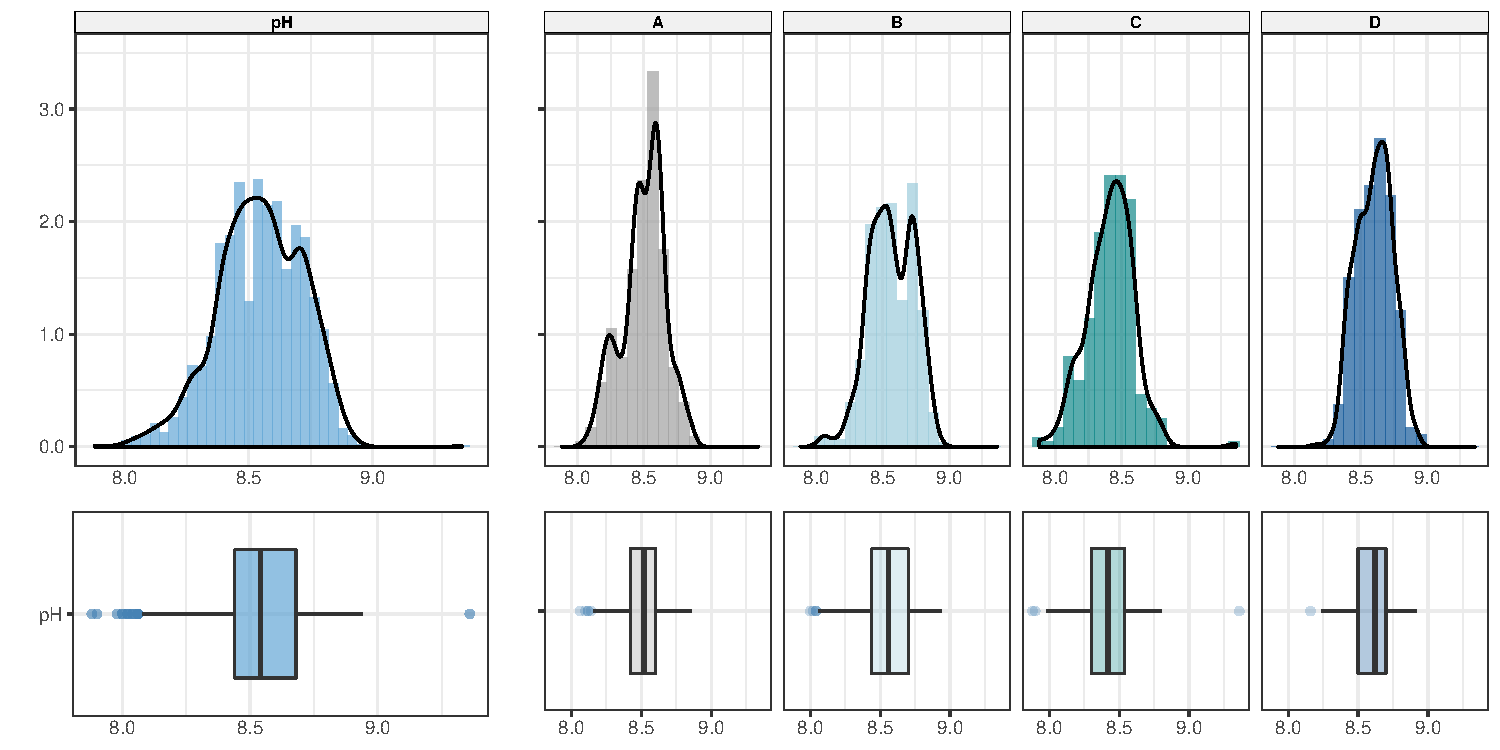
\includegraphics[width=1\textwidth]{Proj2-JM_files/figure-latex/unnamed-chunk-3-1} 

\caption{Distribution of Response Variable: pH}\label{fig:unnamed-chunk-3}
\end{wrapfigure}

Understanding the influence pH has on our predictors is key to building
an accurate predictive model. pH is a measure of acidity/alkalinity that
must conform in a critical range. The value of pH ranges from 0 to 14,
where 0 is acidic, 7 is neutral, and 14 is basic.

Figure 1.1 shows that our response distribution follows a somewhat
normal pattern and is centered around 8.5. The histogram for \texttt{pH}
is bimodal in the aggregate, but varies by brand. The boxplot view
allows us to better visualize the effect outliers have on the skewness
within our target variable.

Brand A has a negatively skewed, multimodal distribution, which could be
suggestive of several distinct underlying response patterns or a higher
degree of variation in \texttt{pH} response for this brand. The density
plot and histogram for Brand B show two bimodal peaks with a slight
positive skew. These peaks indicate that this brand has two distinct
response values that occur more frequently. The distribution for Brand C
and D are both more normal, with a slight negative skew. Brand D has the
highest median \texttt{pH} value and Brand C has the lowest. Brand C
also appears to have the largest spread of \texttt{pH} values.

\hypertarget{predictor-variables}{%
\section{Predictor Variables}\label{predictor-variables}}

We examined the density of our variables to visualize the distribution
of the predictors. Many of these variables contain outliers and present
with a skewed distribution. The outliers fall outside the red-line
boundaries, and highlight which predictors have heavier tails.

The density plots also contain an overlay of the only categorical
indicator, \texttt{BrandCode}. This view shows us that some variables,
including \texttt{AlchRel}, \texttt{CarbRel}, \texttt{CarbVolume},
\texttt{HydPressure4}, and \texttt{Tempature}, are strongly influenced
by brand type.

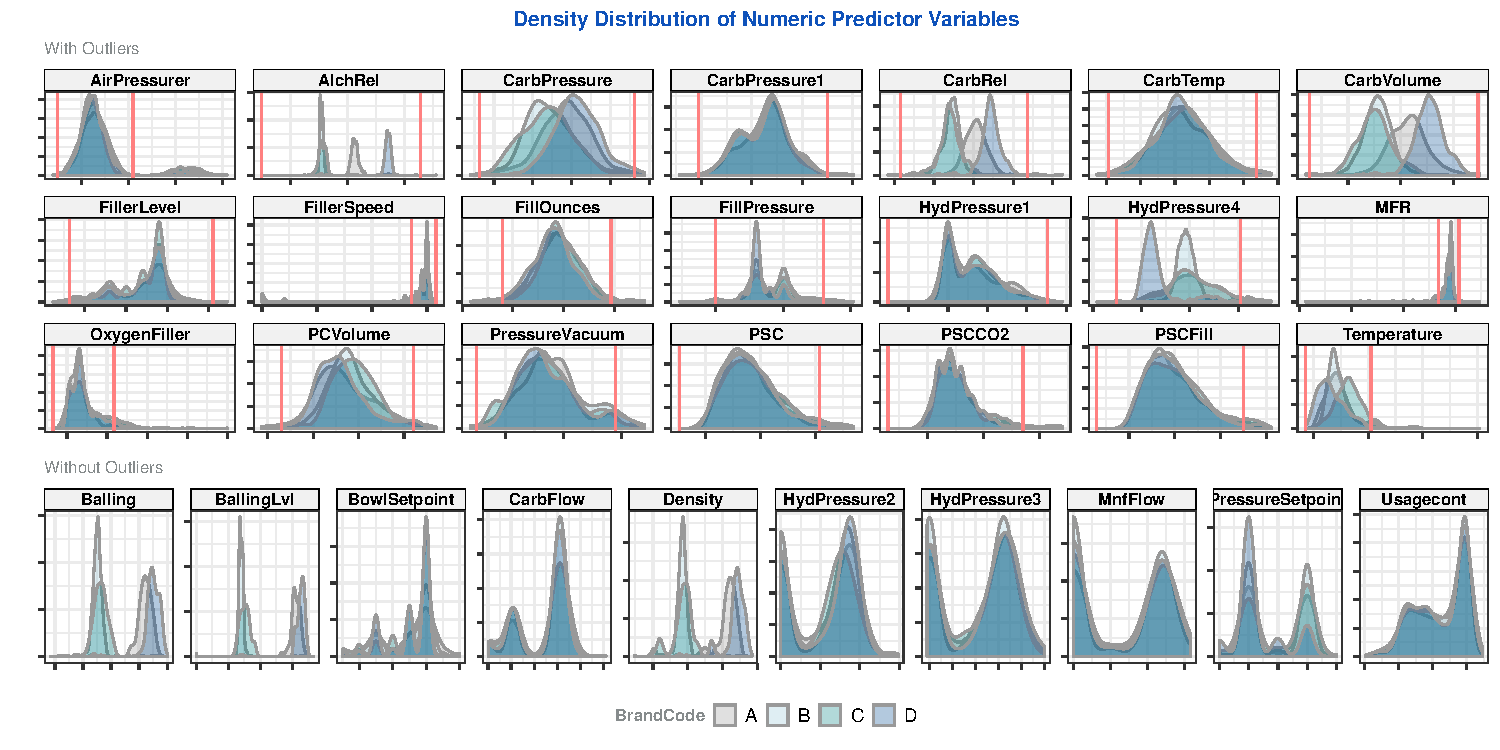
\includegraphics{Proj2-JM_files/figure-latex/unnamed-chunk-4-1.pdf}

We also looked at the relationship of our predictors against the
response variable below. There are a few predictors that have a weak,
linear association with our response variable. However, most of the
indicators show no strong patterns. Given these trends, we do not expect
linear modeling to provide optimal predictions for \texttt{pH}.

This view helps us further visualize the effect \texttt{BrandCode} has
on our predictor and \texttt{pH} values. For example, \texttt{AlchRel}
shows distinct \texttt{BrandCode} groupings. Other variables, such as
\texttt{PSCO2}, \texttt{BowlSetpoint}, \texttt{MinFlow}, and
\texttt{PressureSetup} show unique features likely related to system
processes.

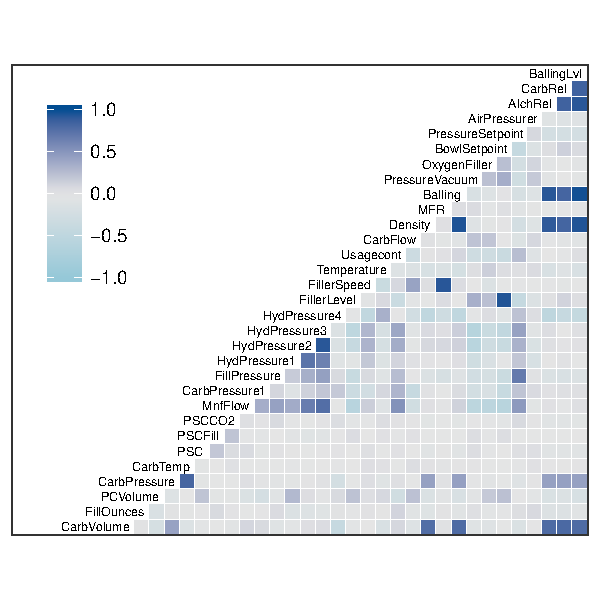
\includegraphics{Proj2-JM_files/figure-latex/unnamed-chunk-5-1.pdf}

Lastly, we examined collinearity measures between our numeric predictors
and found that several of these variables were heavily related, with
correlation values exceeding \(\pm{0.7}\).

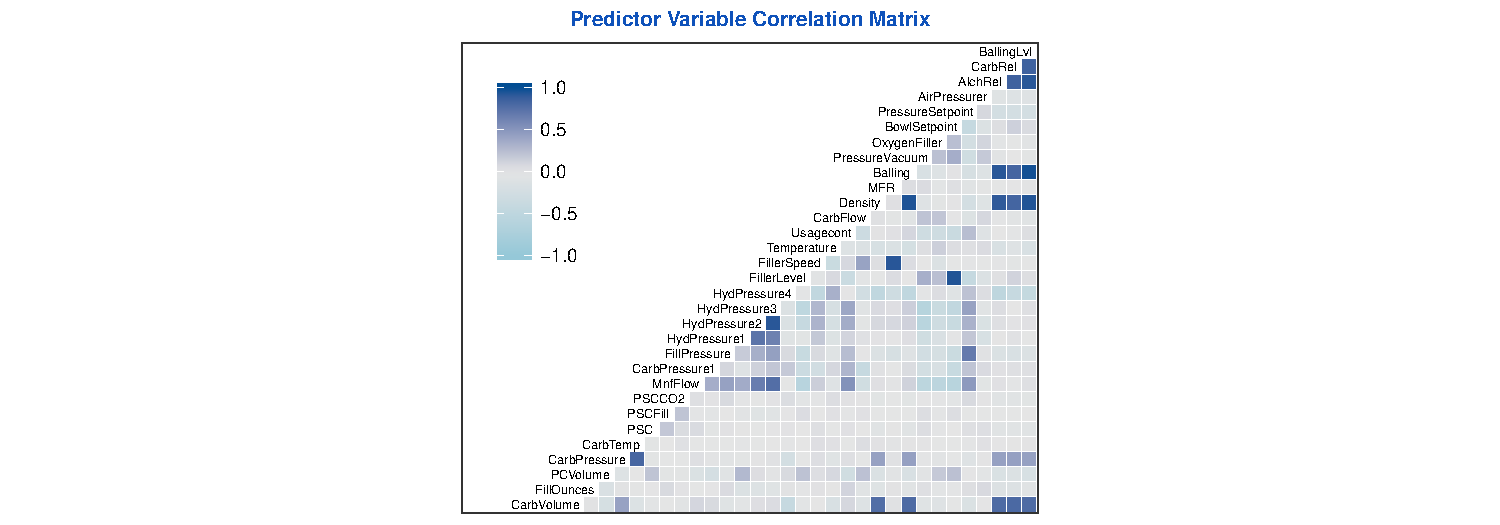
\includegraphics{Proj2-JM_files/figure-latex/unnamed-chunk-6-1.pdf}

\hypertarget{data-preparation}{%
\chapter{Data Preparation}\label{data-preparation}}

In our exploration, we detected missing data, extreme outliers, and
multicollinearity. We kept these factors in mind and applied strategic
transformations when preparing our models to evaluate their performance
with and without normalization changes.

\textbf{Train/Test Splits:}

We divided the production dataset using an 80/20 split to create a train
and test set. All models incorporated k-folds cross-validation set at 10
folds to protect against overfitting the data. We set up unique model
tuning grids to find the optimal parameters for each regression type to
ensure the highest accuracy within our predictions.

\textbf{Data Imputation:}

We applied a Multiple Imputation by Chained Equations (MICE) algorthim
to predict the missing data using sequential regression. This method
filled in all incomplete cases, including \texttt{BrandCode}, our one
unordered categorical variable.

\textbf{Pre-Processing:}

Due to the strong non-normality exhibited in the data, we tested our
models using three different approaches: (1) No pre-processing
techniques, (2) centering and Scaling, and (3) removing zero (and
near-zero) variance and box-cox, centering, and scaling transformations.

\hypertarget{modeling}{%
\chapter{Modeling}\label{modeling}}

We compared the effectiveness of the Multivariate Adaptive Regression
Splines (MARS) to the Elastic Net (eNet) model.

\hypertarget{multivariate-adaptive-regression-splines}{%
\section{Multivariate Adaptive Regression
Splines}\label{multivariate-adaptive-regression-splines}}

MARS modeling was selected to assess the non-linear features in our
data. This method uses a weighted sum to models non-linearities and
interactions between variables. The model assesses cut-points between
features that create the smallest error and prunes insignificant points
to improve model accuracy.

Our RMSE Cross Validation plots show us that pre-processing
transformations did not have improve the MARS model. The model performed
best on our training data when no transformations were applied.

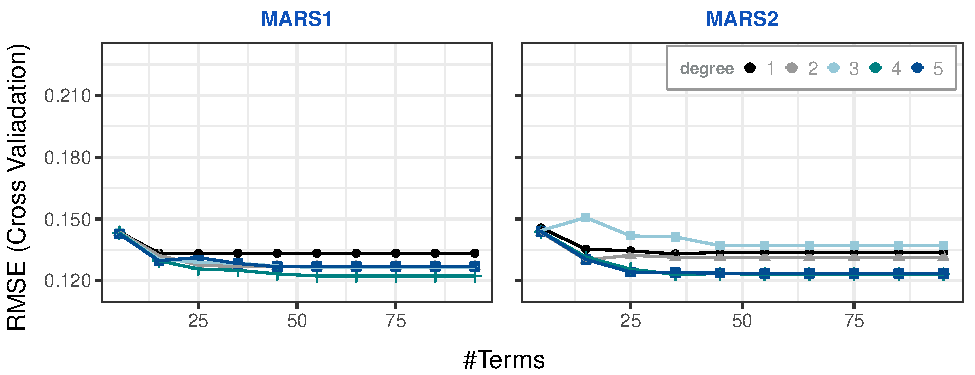
\includegraphics{Proj2-JM_files/figure-latex/unnamed-chunk-7-1.pdf}

\hypertarget{elastic-net}{%
\section{Elastic Net}\label{elastic-net}}

The Elastic Net model was used as it can handle a large number of
predictor variables. It combines ridge and lasso regression techniques
to reduce the size of coefficients. Our RMSE Cross Validation plots show
us that the best tune for both eNET were also similiar, with eNET3
performing the best. The third version of this model incorporated all
pre-processing methods.

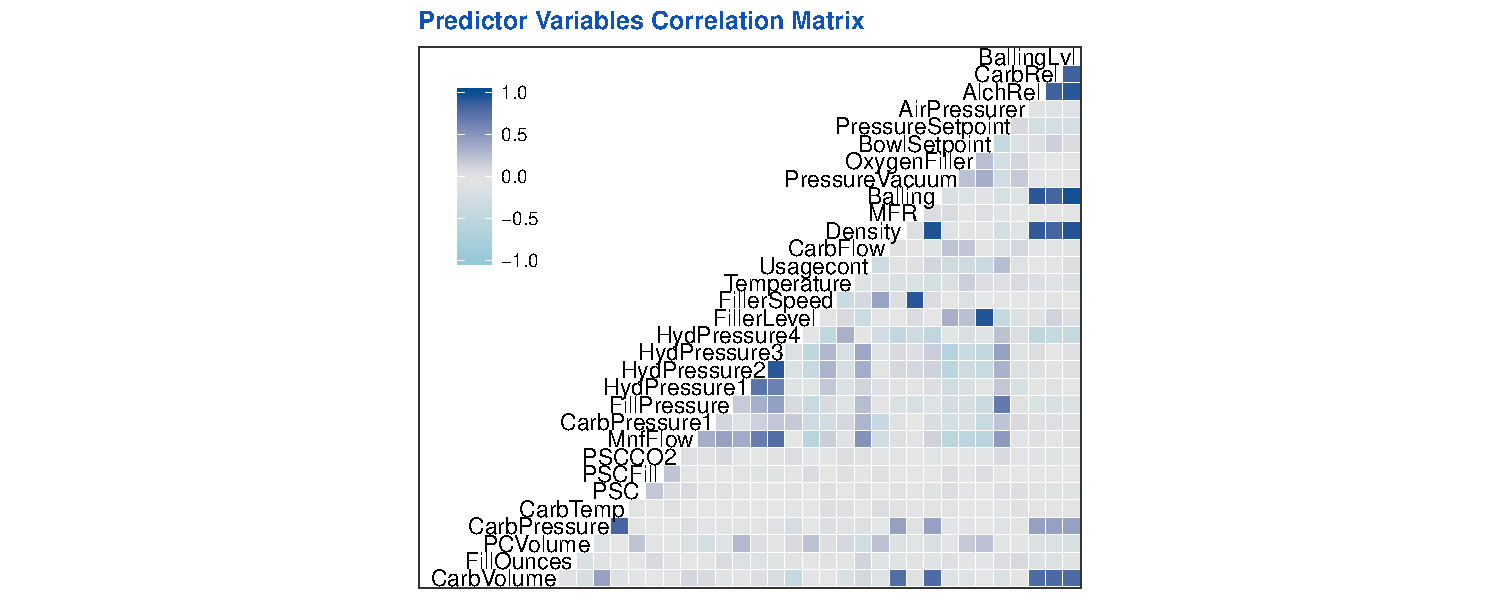
\includegraphics{Proj2-JM_files/figure-latex/unnamed-chunk-8-1.pdf}

\hypertarget{regression-analysis}{%
\chapter{Regression Analysis}\label{regression-analysis}}

\hypertarget{accuracy}{%
\subsubsection{Accuracy}\label{accuracy}}

The MARS model performed the best with the lowest accuracy scores. The
MARS model fit the data the best with the lowest variation between
predicted and observed data for both the training and the test set.

\begin{table}[H]

\caption{\label{tab:unnamed-chunk-9}Accuracy Measures}
\centering
\fontsize{8}{10}\selectfont
\begin{tabular}{l>{\bfseries\leavevmode\color[HTML]{0074D9}}r>{\bfseries\leavevmode\color[HTML]{0074D9}}rrr}
\toprule
  & MARS\_Train & MARS\_Test & eNET\_Train & eNET\_Test\\
\midrule
\rowcolor{gray!6}  RMSE & 0.11978 & 0.12432 & 0.13150 & 0.13506\\
Rsquared & 0.52474 & 0.49261 & 0.41769 & 0.39995\\
\rowcolor{gray!6}  MAE & 0.08950 & 0.09487 & 0.10261 & 0.10643\\
MAPE & 0.01157 & 0.01114 & 0.01280 & 0.01249\\
\bottomrule
\end{tabular}
\end{table}

\hypertarget{variable-importance}{%
\subsubsection{Variable Importance}\label{variable-importance}}

Variable importance varied greatly between the two models. The
predictors, \texttt{MnfFlow}, \texttt{HydPressure3},
\texttt{Useagecont}, and \texttt{BowelSetpoint}, both ranked in the top
10 important variables for MARS and eNET model.

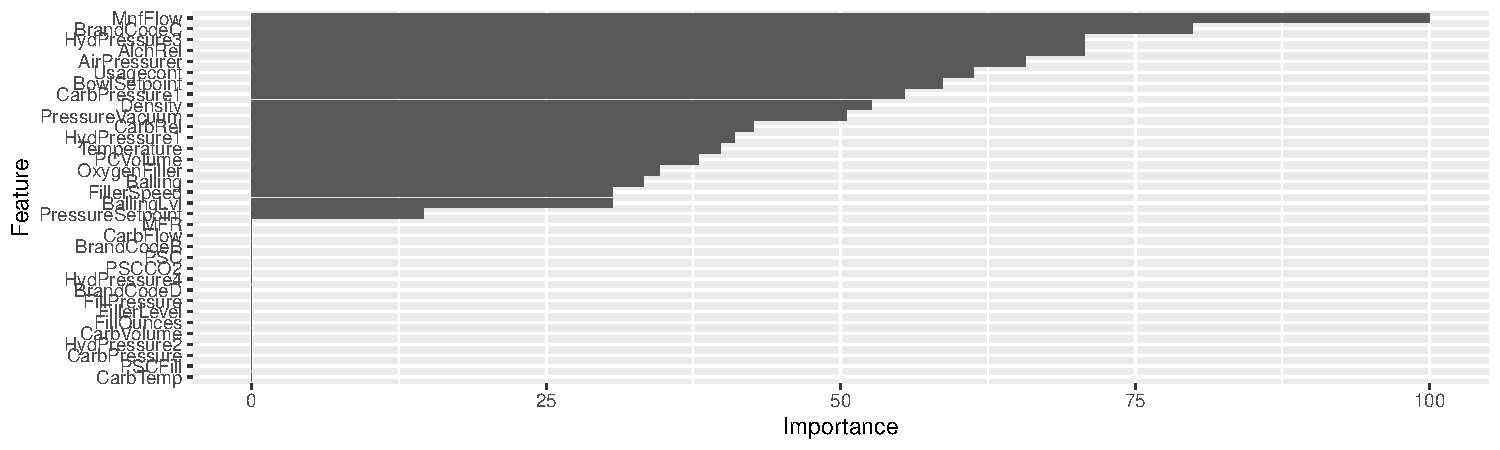
\includegraphics{Proj2-JM_files/figure-latex/unnamed-chunk-10-1.pdf}

\hypertarget{conclusion}{%
\chapter{Conclusion}\label{conclusion}}

This section should contain final thoughts and save/discuss our student
evaluation predictions.

\hypertarget{Appendix}{%
\chapter*{Appendix}\label{Appendix}}
\addcontentsline{toc}{chapter}{Appendix}

\begin{Shaded}
\begin{Highlighting}[]
\KeywordTok{library}\NormalTok{(tidyverse)}
\KeywordTok{library}\NormalTok{(readxl)}
\KeywordTok{library}\NormalTok{(psych)}
\KeywordTok{library}\NormalTok{(mice)}
\KeywordTok{library}\NormalTok{(xtable)}
\KeywordTok{library}\NormalTok{(caret)}
\KeywordTok{library}\NormalTok{(data.table)}
\KeywordTok{library}\NormalTok{(Metrics)}

\CommentTok{# SEEDING}
\KeywordTok{set.seed}\NormalTok{(}\DecValTok{58677}\NormalTok{)}

\CommentTok{# CUSTOM FUNCTIONS}
\NormalTok{gather_if <-}\StringTok{ }\ControlFlowTok{function}\NormalTok{(data, FUN, }\DataTypeTok{key =} \StringTok{"key"}\NormalTok{, }\DataTypeTok{value =} \StringTok{"value"}\NormalTok{, }
 \DataTypeTok{na.rm =} \OtherTok{FALSE}\NormalTok{, }\DataTypeTok{convert =} \OtherTok{FALSE}\NormalTok{, }\DataTypeTok{factor_key =} \OtherTok{FALSE}\NormalTok{) \{}
\NormalTok{ data }\OperatorTok\StringTok{ }\NormalTok{\{}
  \KeywordTok{gather}\NormalTok{(., }\DataTypeTok{key =}\NormalTok{ key, }\DataTypeTok{value =}\NormalTok{ value, }\KeywordTok{names}\NormalTok{(.)[}\KeywordTok{sapply}\NormalTok{(., }
   \DataTypeTok{FUN =}\NormalTok{ FUN)], }\DataTypeTok{na.rm =}\NormalTok{ na.rm, }\DataTypeTok{convert =}\NormalTok{ convert, }
   \DataTypeTok{factor_key =}\NormalTok{ factor_key)}
\NormalTok{ \}}
\NormalTok{\}}

\NormalTok{flattenCorrMatrix <-}\StringTok{ }\ControlFlowTok{function}\NormalTok{(cormat) \{}
\NormalTok{ ut <-}\StringTok{ }\KeywordTok{upper.tri}\NormalTok{(cormat)}
 \KeywordTok{data.table}\NormalTok{(}\DataTypeTok{row =} \KeywordTok{rownames}\NormalTok{(cormat)[}\KeywordTok{row}\NormalTok{(cormat)[ut]], }\DataTypeTok{column =} \KeywordTok{rownames}\NormalTok{(cormat)[}\KeywordTok{col}\NormalTok{(cormat)[ut]], }
  \DataTypeTok{cor =}\NormalTok{ (cormat)[ut])}
\NormalTok{\}}

\CommentTok{# DATA EXPLORATION Import data}
\NormalTok{StudentData <-}\StringTok{ }\KeywordTok{read_xlsx}\NormalTok{(}\StringTok{"~/GitHub/CUNY_DATA_624/Project_Two/data/StudentData.xlsx"}\NormalTok{)}
\NormalTok{StudentEvaluation <-}\StringTok{ }\KeywordTok{read_xlsx}\NormalTok{(}\StringTok{"~/GitHub/CUNY_DATA_624/Project_Two/data/StudentEvaluation.xlsx"}\NormalTok{)}

\CommentTok{## Data Tidying}
\KeywordTok{names}\NormalTok{(StudentData) <-}\StringTok{ }\KeywordTok{gsub}\NormalTok{(}\StringTok{" "}\NormalTok{, }\StringTok{""}\NormalTok{, }\KeywordTok{names}\NormalTok{(StudentData))}
\NormalTok{StudentData <-}\StringTok{ }\NormalTok{StudentData }\OperatorTok\StringTok{ }\KeywordTok{mutate}\NormalTok{(}\DataTypeTok{BrandCode =} \KeywordTok{as.factor}\NormalTok{(BrandCode))}

\CommentTok{## Summary Stats}
\NormalTok{summary_stats <-}\StringTok{ }\KeywordTok{describe}\NormalTok{(StudentData)}

\CommentTok{## Missing Data Analysis}
\NormalTok{MissingData <-}\StringTok{ }\NormalTok{StudentData }\OperatorTok\StringTok{ }\KeywordTok{summarise_all}\NormalTok{(}\KeywordTok{funs}\NormalTok{(}\KeywordTok{sum}\NormalTok{(}\KeywordTok{is.na}\NormalTok{(.)))) }\OperatorTok\StringTok{ }
\StringTok{ }\KeywordTok{t}\NormalTok{() }\OperatorTok\StringTok{ }\KeywordTok{as.data.frame}\NormalTok{() }\OperatorTok\StringTok{ }\KeywordTok{rename}\NormalTok{(}\DataTypeTok{n =}\NormalTok{ V1) }\OperatorTok\StringTok{ }\KeywordTok{rownames_to_column}\NormalTok{(}\StringTok{"predictor"}\NormalTok{) }\OperatorTok\StringTok{ }
\StringTok{ }\KeywordTok{arrange}\NormalTok{(}\KeywordTok{desc}\NormalTok{(n)) }\OperatorTok\StringTok{ }\KeywordTok{mutate}\NormalTok{(}\StringTok{`}\DataTypeTok{%}\StringTok{`}\NormalTok{ =}\StringTok{ }\KeywordTok{round}\NormalTok{((n}\OperatorTok{/}\KeywordTok{nrow}\NormalTok{(StudentData) }\OperatorTok{*}\StringTok{ }
\StringTok{ }\DecValTok{100}\NormalTok{), }\DecValTok{2}\NormalTok{))}

\CommentTok{## Outiers Analysis}
\NormalTok{outliers <-}\StringTok{ }\NormalTok{StudentData }\OperatorTok\StringTok{ }\KeywordTok{mutate}\NormalTok{(}\DataTypeTok{PH =} \KeywordTok{as.factor}\NormalTok{(PH)) }\OperatorTok\StringTok{ }
\StringTok{ }\KeywordTok{gather_if}\NormalTok{(is.numeric, }\StringTok{"key"}\NormalTok{, }\StringTok{"value"}\NormalTok{) }\OperatorTok\StringTok{ }\KeywordTok{filter}\NormalTok{(}\OperatorTok{!}\KeywordTok{is.na}\NormalTok{(value)) }\OperatorTok\StringTok{ }
\StringTok{ }\KeywordTok{group_by}\NormalTok{(key) }\OperatorTok\StringTok{ }\KeywordTok{mutate}\NormalTok{(}\DataTypeTok{outlier_lower =} \KeywordTok{quantile}\NormalTok{(value, }
 \DataTypeTok{probs =} \FloatTok{0.25}\NormalTok{, }\DataTypeTok{na.rm =}\NormalTok{ T) }\OperatorTok{-}\StringTok{ }\FloatTok{1.5} \OperatorTok{*}\StringTok{ }\KeywordTok{IQR}\NormalTok{(value, }\DataTypeTok{na.rm =}\NormalTok{ T), }
 \DataTypeTok{outlier_upper =} \FloatTok{1.5} \OperatorTok{*}\StringTok{ }\KeywordTok{IQR}\NormalTok{(value, }\DataTypeTok{na.rm =}\NormalTok{ T) }\OperatorTok{+}\StringTok{ }\KeywordTok{quantile}\NormalTok{(value, }
  \DataTypeTok{probs =} \FloatTok{0.75}\NormalTok{, }\DataTypeTok{na.rm =}\NormalTok{ T), }\DataTypeTok{outlier =} \KeywordTok{ifelse}\NormalTok{(value }\OperatorTok{<}\StringTok{ }
\StringTok{  }\NormalTok{outlier_lower, }\StringTok{"TRUE"}\NormalTok{, }\KeywordTok{ifelse}\NormalTok{(value }\OperatorTok{>}\StringTok{ }\NormalTok{outlier_upper, }
  \StringTok{"TRUE"}\NormalTok{, }\StringTok{"FALSE"}\NormalTok{)))}
\NormalTok{outlier_with <-}\StringTok{ }\NormalTok{outliers }\OperatorTok\StringTok{ }\KeywordTok{filter}\NormalTok{(}\KeywordTok{any}\NormalTok{(outlier }\OperatorTok{==}\StringTok{ "TRUE"}\NormalTok{)) }\OperatorTok\StringTok{ }
\StringTok{ }\KeywordTok{filter}\NormalTok{(}\OperatorTok{!}\KeywordTok{is.na}\NormalTok{(BrandCode))}
\NormalTok{outlier_wo <-}\StringTok{ }\NormalTok{outliers }\OperatorTok\StringTok{ }\KeywordTok{filter}\NormalTok{(}\KeywordTok{all}\NormalTok{(outlier }\OperatorTok{!=}\StringTok{ "TRUE"}\NormalTok{)) }\OperatorTok\StringTok{ }
\StringTok{ }\KeywordTok{filter}\NormalTok{(}\OperatorTok{!}\KeywordTok{is.na}\NormalTok{(BrandCode))}
\NormalTok{outlier_freq <-}\StringTok{ }\NormalTok{outliers }\OperatorTok\StringTok{ }\KeywordTok{select}\NormalTok{(key, outlier) }\OperatorTok\StringTok{ }\KeywordTok{table}\NormalTok{() }\OperatorTok\StringTok{ }
\StringTok{ }\KeywordTok{as.data.frame.array}\NormalTok{() }\OperatorTok\StringTok{ }\KeywordTok{rownames_to_column}\NormalTok{(}\StringTok{"variable"}\NormalTok{) }\OperatorTok\StringTok{ }
\StringTok{ }\KeywordTok{arrange}\NormalTok{(}\KeywordTok{desc}\NormalTok{(}\StringTok{`}\DataTypeTok{TRUE}\StringTok{`}\NormalTok{)) }\OperatorTok\StringTok{ }\KeywordTok{mutate}\NormalTok{(}\StringTok{`}\DataTypeTok{%}\StringTok{`}\NormalTok{ =}\StringTok{ }\KeywordTok{round}\NormalTok{(}\StringTok{`}\DataTypeTok{TRUE}\StringTok{`}\OperatorTok{/}\NormalTok{(}\StringTok{`}\DataTypeTok{FALSE}\StringTok{`} \OperatorTok{+}\StringTok{ }
\StringTok{ `}\DataTypeTok{TRUE}\StringTok{`}\NormalTok{) }\OperatorTok{*}\StringTok{ }\DecValTok{100}\NormalTok{, }\DecValTok{2}\NormalTok{)) }\OperatorTok\StringTok{ }\KeywordTok{top_n}\NormalTok{(}\DecValTok{5}\NormalTok{, }\StringTok{`}\DataTypeTok{%}\StringTok{`}\NormalTok{)}

\CommentTok{## Correlation}
\NormalTok{cor <-}\StringTok{ }\NormalTok{StudentData }\OperatorTok\StringTok{ }\KeywordTok{select}\NormalTok{(}\OperatorTok{-}\NormalTok{PH, }\OperatorTok{-}\NormalTok{BrandCode) }\OperatorTok\StringTok{ }\KeywordTok{cor}\NormalTok{(}\DataTypeTok{use =} \StringTok{"pairwise.complete.obs"}\NormalTok{)}
\NormalTok{cor_freq <-}\StringTok{ }\KeywordTok{findCorrelation}\NormalTok{(cor, }\FloatTok{0.7}\NormalTok{, }\DataTypeTok{names =}\NormalTok{ T)}
\NormalTok{cor_flat <-}\StringTok{ }\KeywordTok{flattenCorrMatrix}\NormalTok{(cor) }\OperatorTok\StringTok{ }\KeywordTok{arrange}\NormalTok{(row, }\KeywordTok{desc}\NormalTok{(cor)) }\OperatorTok\StringTok{ }
\StringTok{ }\KeywordTok{filter}\NormalTok{(cor }\OperatorTok{>}\StringTok{ }\FloatTok{0.75} \OperatorTok{|}\StringTok{ }\NormalTok{cor }\OperatorTok{<}\StringTok{ }\FloatTok{-0.75}\NormalTok{)}
\NormalTok{cor_flat_left <-}\StringTok{ }\NormalTok{cor_flat }\OperatorTok\StringTok{ }\KeywordTok{slice}\NormalTok{(}\DecValTok{1}\OperatorTok{:}\DecValTok{10}\NormalTok{) }\OperatorTok\StringTok{ }\KeywordTok{mutate}\NormalTok{(}\DataTypeTok{id =} \KeywordTok{row_number}\NormalTok{())}
\NormalTok{cor_flat_right <-}\StringTok{ }\NormalTok{cor_flat }\OperatorTok\StringTok{ }\KeywordTok{slice}\NormalTok{(}\DecValTok{11}\OperatorTok{:}\DecValTok{20}\NormalTok{) }\OperatorTok\StringTok{ }\KeywordTok{mutate}\NormalTok{(}\DataTypeTok{id =} \KeywordTok{row_number}\NormalTok{())}

\CommentTok{# DATA PREPARATION}

\CommentTok{## Imputation}
\NormalTok{init <-}\StringTok{ }\KeywordTok{mice}\NormalTok{(StudentData, }\DataTypeTok{maxit =} \DecValTok{0}\NormalTok{)}
\NormalTok{meth <-}\StringTok{ }\NormalTok{init}\OperatorTok{$}\NormalTok{method}
\NormalTok{predM <-}\StringTok{ }\NormalTok{init}\OperatorTok{$}\NormalTok{predictorMatrix}
\NormalTok{meth[}\KeywordTok{c}\NormalTok{(}\StringTok{"BrandCode"}\NormalTok{)] =}\StringTok{ "polyreg"}
\NormalTok{imputed <-}\StringTok{ }\KeywordTok{mice}\NormalTok{(StudentData, }\DataTypeTok{method =}\NormalTok{ meth, }\DataTypeTok{predictorMatrix =}\NormalTok{ predM, }
 \DataTypeTok{m =} \DecValTok{5}\NormalTok{, }\DataTypeTok{printFlag =}\NormalTok{ F)}
\NormalTok{BevData <-}\StringTok{ }\KeywordTok{complete}\NormalTok{(imputed)}

\CommentTok{## Train/Test Splits}
\NormalTok{trainingRows <-}\StringTok{ }\KeywordTok{createDataPartition}\NormalTok{(BevData}\OperatorTok{$}\NormalTok{PH, }\DataTypeTok{p =} \FloatTok{0.8}\NormalTok{, }
 \DataTypeTok{list =} \OtherTok{FALSE}\NormalTok{)}

\CommentTok{## Split Train/Test Data}
\NormalTok{train <-}\StringTok{ }\NormalTok{BevData[trainingRows, ]}
\NormalTok{test <-}\StringTok{ }\NormalTok{BevData[}\OperatorTok{-}\NormalTok{trainingRows, ]}

\CommentTok{# MODELING}
\NormalTok{tl <-}\StringTok{ }\DecValTok{5}
\NormalTok{trC <-}\StringTok{ }\KeywordTok{trainControl}\NormalTok{(}\DataTypeTok{method =} \StringTok{"cv"}\NormalTok{, }\DataTypeTok{number =} \DecValTok{10}\NormalTok{, }\DataTypeTok{savePredictions =}\NormalTok{ T)}

\CommentTok{## MARS}
\NormalTok{mars_grid <-}\StringTok{ }\KeywordTok{expand.grid}\NormalTok{(}\DataTypeTok{degree =} \DecValTok{1}\OperatorTok{:}\DecValTok{3}\NormalTok{, }\DataTypeTok{nprune =} \KeywordTok{seq}\NormalTok{(}\DecValTok{5}\NormalTok{, }\DecValTok{50}\NormalTok{, }
 \DataTypeTok{by =} \DecValTok{10}\NormalTok{))}
\NormalTok{mars_fit1 <-}\StringTok{ }\KeywordTok{train}\NormalTok{(PH }\OperatorTok{~}\StringTok{ }\NormalTok{., }\DataTypeTok{data =}\NormalTok{ train, }\DataTypeTok{method =} \StringTok{"earth"}\NormalTok{, }
 \DataTypeTok{tuneGrid =}\NormalTok{ mars_grid, }\DataTypeTok{trControl =}\NormalTok{ trC, }\DataTypeTok{tuneLength =}\NormalTok{ tl)}
\NormalTok{mars_fit2 <-}\StringTok{ }\KeywordTok{train}\NormalTok{(PH }\OperatorTok{~}\StringTok{ }\NormalTok{., }\DataTypeTok{data =}\NormalTok{ train, }\DataTypeTok{method =} \StringTok{"earth"}\NormalTok{, }
 \DataTypeTok{preProcess =} \KeywordTok{c}\NormalTok{(}\StringTok{"center"}\NormalTok{, }\StringTok{"scale"}\NormalTok{), }\DataTypeTok{tuneGrid =}\NormalTok{ mars_grid, }
 \DataTypeTok{trControl =}\NormalTok{ trC, }\DataTypeTok{tuneLength =}\NormalTok{ tl)}
\NormalTok{mars_fit3 <-}\StringTok{ }\KeywordTok{train}\NormalTok{(PH }\OperatorTok{~}\StringTok{ }\NormalTok{., }\DataTypeTok{data =}\NormalTok{ train, }\DataTypeTok{method =} \StringTok{"earth"}\NormalTok{, }
 \DataTypeTok{preProcess =} \KeywordTok{c}\NormalTok{(}\StringTok{"nzv"}\NormalTok{, }\StringTok{"zv"}\NormalTok{, }\StringTok{"BoxCox"}\NormalTok{, }\StringTok{"center"}\NormalTok{, }\StringTok{"scale"}\NormalTok{), }
 \DataTypeTok{tuneGrid =}\NormalTok{ mars_grid, }\DataTypeTok{trControl =}\NormalTok{ trC, }\DataTypeTok{tuneLength =}\NormalTok{ tl)}

\NormalTok{mars_test_pred1 <-}\StringTok{ }\KeywordTok{predict}\NormalTok{(mars_fit1, }\DataTypeTok{newdata =}\NormalTok{ test)}
\NormalTok{mars_test_pred2 <-}\StringTok{ }\KeywordTok{predict}\NormalTok{(mars_fit2, }\DataTypeTok{newdata =}\NormalTok{ test)}
\NormalTok{mars_test_pred3 <-}\StringTok{ }\KeywordTok{predict}\NormalTok{(mars_fit2, }\DataTypeTok{newdata =}\NormalTok{ test)}

\CommentTok{## eNET}
\NormalTok{enet_grid <-}\StringTok{ }\KeywordTok{expand.grid}\NormalTok{(}\DataTypeTok{lambda =} \KeywordTok{c}\NormalTok{(}\DecValTok{0}\NormalTok{, }\FloatTok{0.05}\NormalTok{, }\FloatTok{0.1}\NormalTok{), }\DataTypeTok{fraction =} \KeywordTok{seq}\NormalTok{(}\FloatTok{0.05}\NormalTok{, }
 \DecValTok{1}\NormalTok{, }\DataTypeTok{length =} \DecValTok{20}\NormalTok{))}
\NormalTok{enet_fit1 <-}\StringTok{ }\KeywordTok{train}\NormalTok{(PH }\OperatorTok{~}\StringTok{ }\NormalTok{., }\DataTypeTok{data =}\NormalTok{ train, }\DataTypeTok{method =} \StringTok{"enet"}\NormalTok{, }
 \DataTypeTok{metric =} \StringTok{"RMSE"}\NormalTok{, }\DataTypeTok{tuneGrid =}\NormalTok{ enet_grid, }\DataTypeTok{tuneLength =}\NormalTok{ tl, }
 \DataTypeTok{trControl =}\NormalTok{ trC)}
\NormalTok{enet_fit2 <-}\StringTok{ }\KeywordTok{train}\NormalTok{(PH }\OperatorTok{~}\StringTok{ }\NormalTok{., }\DataTypeTok{data =}\NormalTok{ train, }\DataTypeTok{method =} \StringTok{"enet"}\NormalTok{, }
 \DataTypeTok{preProcess =} \KeywordTok{c}\NormalTok{(}\StringTok{"center"}\NormalTok{, }\StringTok{"scale"}\NormalTok{), }\DataTypeTok{metric =} \StringTok{"RMSE"}\NormalTok{, }\DataTypeTok{tuneGrid =}\NormalTok{ enet_grid, }
 \DataTypeTok{tuneLength =}\NormalTok{ tl, }\DataTypeTok{trControl =}\NormalTok{ trC)}
\NormalTok{enet_fit3 <-}\StringTok{ }\KeywordTok{train}\NormalTok{(PH }\OperatorTok{~}\StringTok{ }\NormalTok{., }\DataTypeTok{data =}\NormalTok{ train, }\DataTypeTok{method =} \StringTok{"enet"}\NormalTok{, }
 \DataTypeTok{preProcess =} \KeywordTok{c}\NormalTok{(}\StringTok{"nzv"}\NormalTok{, }\StringTok{"zv"}\NormalTok{, }\StringTok{"BoxCox"}\NormalTok{, }\StringTok{"center"}\NormalTok{, }\StringTok{"scale"}\NormalTok{), }
 \DataTypeTok{metric =} \StringTok{"RMSE"}\NormalTok{, }\DataTypeTok{tuneGrid =}\NormalTok{ enet_grid, }\DataTypeTok{trControl =}\NormalTok{ trC, }
 \DataTypeTok{tuneLength =}\NormalTok{ tl)}

\NormalTok{enet_test_pred1 <-}\StringTok{ }\KeywordTok{predict}\NormalTok{(enet_fit1, }\DataTypeTok{newdata =}\NormalTok{ test)}
\NormalTok{enet_test_pred2 <-}\StringTok{ }\KeywordTok{predict}\NormalTok{(enet_fit2, }\DataTypeTok{newdata =}\NormalTok{ test)}
\NormalTok{enet_test_pred3 <-}\StringTok{ }\KeywordTok{predict}\NormalTok{(enet_fit2, }\DataTypeTok{newdata =}\NormalTok{ test)}


\CommentTok{# ACCURACY}
\NormalTok{MARS_MAPE_TRN <-}\StringTok{ }\NormalTok{Metrics}\OperatorTok{::}\KeywordTok{mape}\NormalTok{(mars_fit1}\OperatorTok{$}\NormalTok{pred}\OperatorTok{$}\NormalTok{obs, mars_fit1}\OperatorTok{$}\NormalTok{pred}\OperatorTok{$}\NormalTok{pred)}
\NormalTok{eNET_MAPE_TRN <-}\StringTok{ }\NormalTok{Metrics}\OperatorTok{::}\KeywordTok{mape}\NormalTok{(enet_fit3}\OperatorTok{$}\NormalTok{pred}\OperatorTok{$}\NormalTok{obs, enet_fit3}\OperatorTok{$}\NormalTok{pred}\OperatorTok{$}\NormalTok{pred)}
\NormalTok{MARS_MAPE_TST <-}\StringTok{ }\NormalTok{Metrics}\OperatorTok{::}\KeywordTok{mape}\NormalTok{(test}\OperatorTok{$}\NormalTok{PH, mars_test_pred1)}
\NormalTok{eNET_MAPE_TST <-}\StringTok{ }\NormalTok{Metrics}\OperatorTok{::}\KeywordTok{mape}\NormalTok{(test}\OperatorTok{$}\NormalTok{PH, enet_test_pred3)}
\NormalTok{MARS_PERF_TRN <-}\StringTok{ }\NormalTok{mars_fit1}\OperatorTok{$}\NormalTok{results }\OperatorTok\StringTok{ }\KeywordTok{as.data.frame}\NormalTok{() }\OperatorTok\StringTok{ }
\StringTok{ }\KeywordTok{filter}\NormalTok{(RMSE }\OperatorTok{==}\StringTok{ }\KeywordTok{min}\NormalTok{(RMSE)) }\OperatorTok\StringTok{ }\KeywordTok{select}\NormalTok{(RMSE, Rsquared, }
\NormalTok{ MAE) }\OperatorTok\StringTok{ }\KeywordTok{distinct}\NormalTok{() }\OperatorTok\StringTok{ }\KeywordTok{mutate}\NormalTok{(}\DataTypeTok{Variable =} \StringTok{"MARS_Train"}\NormalTok{) }\OperatorTok\StringTok{ }
\StringTok{ }\KeywordTok{column_to_rownames}\NormalTok{(}\StringTok{"Variable"}\NormalTok{) }\OperatorTok\StringTok{ }\KeywordTok{t}\NormalTok{()}
\NormalTok{eNET_PERF_TRN <-}\StringTok{ }\NormalTok{enet_fit3}\OperatorTok{$}\NormalTok{results }\OperatorTok\StringTok{ }\KeywordTok{as.data.frame}\NormalTok{() }\OperatorTok\StringTok{ }
\StringTok{ }\KeywordTok{filter}\NormalTok{(RMSE }\OperatorTok{==}\StringTok{ }\KeywordTok{min}\NormalTok{(RMSE)) }\OperatorTok\StringTok{ }\KeywordTok{select}\NormalTok{(RMSE, Rsquared, }
\NormalTok{ MAE) }\OperatorTok\StringTok{ }\KeywordTok{distinct}\NormalTok{() }\OperatorTok\StringTok{ }\KeywordTok{mutate}\NormalTok{(}\DataTypeTok{Variable =} \StringTok{"eNET_Train"}\NormalTok{) }\OperatorTok\StringTok{ }
\StringTok{ }\KeywordTok{column_to_rownames}\NormalTok{(}\StringTok{"Variable"}\NormalTok{) }\OperatorTok\StringTok{ }\KeywordTok{t}\NormalTok{()}
\NormalTok{MARS_PERF_TST <-}\StringTok{ }\KeywordTok{postResample}\NormalTok{(}\DataTypeTok{pred =}\NormalTok{ mars_test_pred1, }\DataTypeTok{obs =}\NormalTok{ test}\OperatorTok{$}\NormalTok{PH)}
\NormalTok{eNET_PERF_TST <-}\StringTok{ }\KeywordTok{postResample}\NormalTok{(}\DataTypeTok{pred =}\NormalTok{ enet_test_pred3, }\DataTypeTok{obs =}\NormalTok{ test}\OperatorTok{$}\NormalTok{PH)}
\NormalTok{bind1 <-}\StringTok{ }\KeywordTok{cbind}\NormalTok{(MARS_PERF_TRN, }\DataTypeTok{MARS_Test =}\NormalTok{ MARS_PERF_TST, }
\NormalTok{ eNET_PERF_TRN, }\DataTypeTok{eNET_Test =}\NormalTok{ eNET_PERF_TST)}
\NormalTok{bind2 <-}\StringTok{ }\KeywordTok{cbind}\NormalTok{(MARS_MAPE_TRN, MARS_MAPE_TST, eNET_MAPE_TRN, }
\NormalTok{ eNET_MAPE_TST)}
\KeywordTok{row.names}\NormalTok{(bind2) <-}\StringTok{ "MAPE"}
\NormalTok{Tbl_Accuracy <-}\StringTok{ }\KeywordTok{rbind}\NormalTok{(bind1, bind2)}

\CommentTok{# VARIABLE IMPORTANCE}
\NormalTok{MARS_VarImp <-}\StringTok{ }\KeywordTok{varImp}\NormalTok{(mars_fit1, }\DataTypeTok{scale =}\NormalTok{ T)}
\NormalTok{eNET_VarImp <-}\StringTok{ }\KeywordTok{varImp}\NormalTok{(enet_fit3, }\DataTypeTok{scale =}\NormalTok{ T)}
\end{Highlighting}
\end{Shaded}


\end{document}
